% Created 2021-05-14 Fri 16:44
% Intended LaTeX compiler: pdflatex
\documentclass[presentation]{beamer}
\usepackage[utf8]{inputenc}
\usepackage[T1]{fontenc}
\usepackage{graphicx}
\usepackage{grffile}
\usepackage{longtable}
\usepackage{wrapfig}
\usepackage{rotating}
\usepackage[normalem]{ulem}
\usepackage{amsmath}
\usepackage{textcomp}
\usepackage{amssymb}
\usepackage{capt-of}
\usepackage{hyperref}
\usepackage{minted}
\usepackage[utf8]{inputenc}
\usepackage{color}
\usetheme[height=7mm]{Rochester}
\setbeamertemplate{footline}[frame number]
\usecolortheme[accent=red, light]{solarized}
\setbeamercolor{frametitle}{bg=solarizedRebase02,fg=solarizedAccent}
\setbeamercolor{author in head/foot}{bg=solarizedRebase02,fg=solarizedRebase01}
\setbeamercolor{title in head/foot}{bg=solarizedRebase02,fg=solarizedRebase01}
\setbeamercolor{block title}{bg=solarizedRebase0,fg=solarizedRebase02}
\setbeamercolor{block body}{bg=solarizedRebase02,fg=solarizedRebase0}
\setbeamercolor{item}{bg=solarizedRebase02,fg=solarizedAccent}
\beamertemplatenavigationsymbolsempty
\usemintedstyle{manni}
\AtBeginSection[]{
\begin{frame}
\vfill
\centering
\begin{beamercolorbox}[sep=8pt,center,shadow=true,rounded=true]{title}
\Huge\insertsectionhead\par%
\end{beamercolorbox}
\vfill
\end{frame}
}
\usetheme{default}
\author{Sebastian Stabinger, Thomas Hausberger}
\date{SS2021}
\title{Ausnahmebehandlung}
\hypersetup{
 pdfauthor={Sebastian Stabinger, Thomas Hausberger},
 pdftitle={Ausnahmebehandlung},
 pdfkeywords={},
 pdfsubject={},
 pdfcreator={Emacs 27.2 (Org mode 9.4.5)}, 
 pdflang={Ger}}
\begin{document}

\maketitle

\begin{frame}[label={sec:orgea49bed}]{Was versteht man unter Ausnahmebehandlung?}
\begin{itemize}
\item Ausnahmebehandlung (engl. Exception Handeling) beschreibt die
Methoden und Systeme die man verwendet um mit Fehlern \alert{zur Laufzeit}
umzugehen
\item Wir wollen also nicht, dass unser Programm einfach abstürzt, wir
\alert{wollen auf den Fehler sinnvoll reagieren}
\end{itemize}
\begin{block}{Beispiele}
\begin{itemize}
\item Wir haben eine Division durch Null
\item Wir wollen den Durchschnitt eines Vektors berechnen, aber der Vektor
ist leer
\item Wir öffnen eine Datei zum Lesen, aber die Datei existiert nicht
\item Wir versuchen eine Verbindung zu einem Server aufzubauen, aber der
Server meldet sich nicht
\item \ldots{}
\end{itemize}
\end{block}
\end{frame}
\section{Ausnahmebehandlung in C}
\label{sec:orgdaa5dc8}
\begin{frame}[label={sec:org12ea58b}]{Ausnahmebehandlung in C}
\begin{itemize}
\item In C gibt es \alert{kein spezielles System} um mit Laufzeitfehlern
umzugehen
\item Man muss also \alert{existierende Sprachelemente nutzen}
\end{itemize}
\begin{block}{Möglichkeiten der Fehlerbehandlung:}
\begin{itemize}
\item Über den \alert{Rückgabewert}
\item Über \alert{globale Variablen}
\item Über \alert{einen Zeiger} der als Parameter übergeben wird
\end{itemize}
\end{block}
\end{frame}
\begin{frame}[label={sec:org6d69a5e},fragile]{Beispiel mit Rückgabewert}
 \begin{minted}[fontsize=\scriptsize,numberblanklines=false]{c}
#include <stdio.h>
#include <stdlib.h>

int do_something() {
  if (rand() % 5 == 0)
    return -1; // Ein Fehler ist aufgetreten
  else
    return 0; // Alles OK
}

int main() {
  for (int i = 0; i < 10; i++) {
    int returnvalue = do_something();
    if (returnvalue == 0)
      printf("Alles OK\n");
    else if (returnvalue == -1)
      printf("In do_something ist ein Fehler aufgetreten.\n");
  }
}
\end{minted}
\end{frame}
\begin{frame}[label={sec:orgb3f6ef4},fragile]{Beispiel mit globaler Variable}
 \begin{minted}[fontsize=\scriptsize,numberblanklines=false]{c}
#include <stdio.h>

int sumerror = 0;
int sum(int start, int stop) {
  if (start > stop) {
    sumerror = -1; // Wir haben ein Problem!
    return 0;
  }
  int sum = 0;
  for (int i = start; i <= stop; i++)
    sum += i;
  sumerror = 0; // Alles war ok
  return sum;
}

int main() {
  int s = sum(10, 20);
  if (sumerror == 0) printf("Summe ist %d\n", s);
  else printf("Fehler beim Berechnen der Summer\n");
  s = sum(30, 10);
  if (sumerror == 0) printf("Summe ist %d\n", s);
  else printf("Fehler beim Berechnen der Summer\n");
}
\end{minted}
\end{frame}
\begin{frame}[label={sec:orgceab1e5},fragile]{Beispiel mit Zeiger}
 \begin{minted}[fontsize=\scriptsize,numberblanklines=false]{c}
#include <stdio.h>

int sum(int start, int stop, int *error) {
    if (start > stop) {
        *error = -1; // Wir haben ein Problem!
        return 0;
    }
    int sum = 0;
    for (int i = start; i <= stop; i++)
        sum += i;
    *error = 0; // Alles war ok
    return sum;
}

int main() {
    int sumerror = 0;
    int s = sum(10, 20, &sumerror);
    if (sumerror == 0) printf("Summe ist %d\n", s);
    else printf("Fehler beim Berechnen der Summer\n");
    s = sum(30, 10, &sumerror);
    if (sumerror == 0) printf("Summe ist %d\n", s);
    else printf("Fehler beim Berechnen der Summer\n");
}
\end{minted}
\end{frame}
\begin{frame}[label={sec:orgd3a68f2},fragile]{Vor- und Nachteile der unterschiedlichen Varianten}
 \begin{itemize}
\item \alert{Mit Rückgabewert:} Funktioniert gut, wenn wir den Rückgabewert der
Funktion nicht für etwas anderes benötigen, oder wenn es
Rückgabewerte gibt, die normalerweise nicht vorkommen können.
\item \alert{Mit globaler Variable:} Kann auch verwendet werden, wenn der
Rückgabewert benötigt wird. Unübersichtlich und funktioniert nicht,
wenn die gleiche Funktion parallel öfter aufgerufen wird (was Heute
immer häufiger ist)
\item \alert{Mit Zeiger:} Die sauberste Variante, aber etwas aufwändig, da man
eine Variable erzeugen muss etc.
\end{itemize}
\begin{block}{Genereller Nachteil}
Wir müssen jeden einzelnen Fehler immer manuell mit einer
{\color{solarizedYellow}\texttt{if}}-Bedingung abfangen
\end{block}
\end{frame}
\section{Ausnahmebehandlung in C++}
\label{sec:orgc628c23}
\begin{frame}[label={sec:org9f90b25},fragile]{Überblick}
 \begin{block}{Ausnahme {\color{solarizedYellow}\texttt{exception}}}
Ein beliebiges Objekt. Üblicherweise aber eine \alert{Instanz einer Klasse}
die von der Klasse {\color{solarizedYellow}\texttt{exception} }abgeleitet ist.
\end{block}
\begin{block}{Werfen {\color{solarizedYellow}\texttt{throw}}}
\begin{itemize}
\item Entdecken wir einen Fehler, können wir eine \alert{Ausnahme werfen} (engl.
\emph{to throw an exception})
\end{itemize}
\end{block}
\begin{block}{Fangen {\color{solarizedYellow}\texttt{catch}}}
\begin{itemize}
\item Wir können für einen bestimmten Teil unseres Codes angeben was
passieren soll falls während der Ausführung eine Ausnahme auftritt.
Man spricht davon, dass die \alert{Ausnahme gefangen} wird (engl. \emph{to
catch an exception})
\item Wir können auch angeben \alert{welche Fehler} wir fangen wollen und was bei
unterschiedlichen Fehlern passieren soll
\end{itemize}
\end{block}
\end{frame}
\begin{frame}[label={sec:org5298115},fragile]{Das Werfen einer Ausnahme}
 \begin{itemize}
\item Das Werfen einer Ausnahme geschieht mit dem Schlüsselwort {\color{solarizedYellow}\texttt{throw}}
\item {\color{solarizedYellow}\texttt{throw} }funktioniert ähnlich wie {\color{solarizedYellow}\texttt{return}}, wir müssen uns aber nicht
auf einen Rückgabetyp festlegen
\item Üblicherweise wirft man aber Klassen die von {\color{solarizedYellow}\texttt{std::exception}}
abgeleitet sind
\end{itemize}
\begin{block}{Beispiel}
\begin{minted}[fontsize=\scriptsize,numberblanklines=false]{c++}
void ein_fehler() {
  // Wir haben einfach immer einen Fehler
  throw 23; // Wirft 23 als Ausnahme
}
\end{minted}
Man sieht: Obwohl der Rückgabewert der Funktion {\color{solarizedYellow}\texttt{void} }ist, können wir
mit {\color{solarizedYellow}\texttt{throw} }einen Integer als Ausnahme zurück geben.
\end{block}
\end{frame}
\begin{frame}[label={sec:org48e7459},fragile]{Vordefinierte Exceptions}
 Verfügbar mit {\color{solarizedYellow}\texttt{\#include <exception>}}
\begin{center}\begin{center}
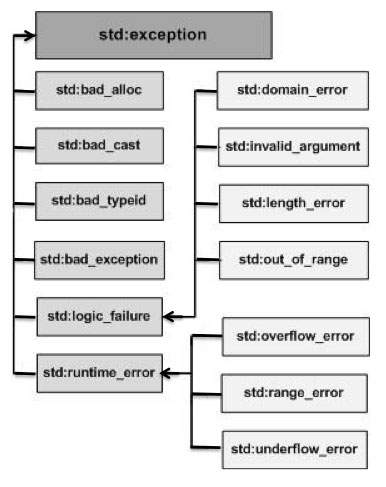
\includegraphics[width=0.5\textwidth]{img/cpp_exceptions.jpg}
\end{center}\end{center}
\tiny
Von \url{https://www.tutorialspoint.com/cplusplus/cpp\_exceptions\_handling.htm}
\end{frame}
\begin{frame}[label={sec:org0f3206c},fragile]{Das Werfen einer Ausnahme}
 \begin{minted}[fontsize=\scriptsize,numberblanklines=false]{c++}
#include <iostream>
#include <exception>
using namespace std;

void ein_fehler() {
  // Wir haben immer einen Fehler
  throw runtime_error("Oh nein, ein Fehler!!");
}

int main() {
    cout << "Alles OK" << endl;
    ein_fehler();
    cout << "Immer noch alles OK" << endl;
}
\end{minted}
\begin{itemize}
\item Man kann einer Ausnahme üblicherweise einen \alert{String} mitgeben der
\alert{näher erklärt} was genau passiert ist
\item Wenn man eine \alert{Ausnahme nicht fängt}, \alert{stürzt das Programm ab} und
man erfährt welche Ausnahme dafür verantwortlich war und welchen
String sie enthalten hat
\end{itemize}
\end{frame}
\begin{frame}[label={sec:org57c8ac0},fragile]{Das Fangen einer allgemeinen Ausnahme}
 \begin{itemize}
\item Das Stück Code in dem eine Ausnahme gefangen werden soll wird in ein
{\color{solarizedYellow}\texttt{try \{ \}} }eingeschlossen
\item Anschließend wird mit {\color{solarizedYellow}\texttt{catch(...) \{ \}} }angegeben \alert{welcher Code} im
Fall einer Ausnahme ausgeführt werden soll
\end{itemize}
\begin{block}{Beispiel}
\begin{minted}[fontsize=\scriptsize,numberblanklines=false]{c++}
try {
  cout << "Alles OK" << endl;
  eine_funktion();
  cout << "Immer noch alles OK" << endl;
} catch (...) {
  cout << "Ouch: Irgendwo oben gab es eine Ausnahme!" << endl;
}
\end{minted}
\end{block}
\end{frame}
\begin{frame}[label={sec:org3aef413},fragile]{Das Fangen einer speziellen Ausnahme}
 \begin{itemize}
\item {\color{solarizedYellow}\texttt{catch(...)} }bedeutet, dass bei \alert{jeder Ausnahme} reagiert werden
soll
\item Falls wir nur auf \alert{spezielle Ausnahmen} reagieren wollen schreiben
wir in die Klammern \alert{welche Ausnahme} das sein soll und wie das
Ausnahmeobjekt bezeichnet werden soll
\item Wir können mehrere {\color{solarizedYellow}\texttt{catch} }Anweisungen hintereinander hängen
\end{itemize}
\begin{block}{Beispiel}
\begin{minted}[fontsize=\scriptsize,numberblanklines=false]{c++}
try {
  cout << "Alles OK" << endl;
  eine_funktion();
  cout << "Immer noch alles OK" << endl;
} catch (overflow_error &e) {
  cout << "Ouch: Irgendwo oben gab es einen runtime_error!" << endl;
  cout << "Nachricht war: " << e.what() << endl;
} catch (range_error &e) {
    cout << "Ouch: Irgendwo oben gab es einen range_error!" << endl;
    cout << "Nachricht war: " << e.what() << endl;
}
\end{minted}
\end{block}
\end{frame}
\begin{frame}[label={sec:orgd1a55b6},fragile]{Beispiel}
 \begin{minted}[fontsize=\scriptsize,numberblanklines=false]{c++}
#include <exception>
#include <iostream>
using namespace std;

void do_something() {
  if (rand() % 5 == 0)
    throw runtime_error("We got a 0, and we don't like it!");
}

int main() {
  for (int i = 0; i < 10; i++) {
    try {
      do_something();
      cout << "Alles OK!" << endl;
    } catch (exception &e) {
      cout << "Some error occured with the message: " << endl;
      cout << e.what() << endl;
    }
  }
}
\end{minted}
\end{frame}
\begin{frame}[label={sec:org45d4965},fragile]{Übung}
 \begin{itemize}
\item Implementieren Sie Ihre \alert{eigene Divisionsfunktion} {\color{solarizedYellow}\texttt{double
  mydiv(double a, double b)} }welche das Ergebnis von {\color{solarizedYellow}\texttt{a} }geteilt durch
{\color{solarizedYellow}\texttt{b} }zurück gibt.
\item Falls eine Division durch 0 droht, soll die Funktion eine Ausnahme
({\color{solarizedYellow}\texttt{domain\_error}}) zurück liefern.
\item Testen Sie ihren Code an ein paar Beispielen und fangen Sie mögliche
Ausnahmen mit {\color{solarizedYellow}\texttt{try} }und {\color{solarizedYellow}\texttt{catch} }ab
\end{itemize}
\end{frame}
\end{document}